\chapter{Question 4}
\label{available-representation}

\textbf{Repeat A3, Q1.  Compare the resulting text from February to the text you have now.  Do all 1000 URIs still return a ``200 OK'' as their final response (i.e., at the end of possible redirects)?\\\\
Create two graphs similar to that described in Q3, except this time the y-axis corresponds to difference in bytes (and not difference in TimeMap magnitudes).  For the first graph, use the difference in the raw (unprocessed) results.  For the second graph, use the  difference in the processed (as per A3, Q1) results.\\\\
Of the URIs that still terminate in a ``200 OK'' response, pick the top 3 most changed (processed) pairs of pages and use the Unix ``diff'' command to explore the differences in the version pairs.}\\\\

Following are the steps I have taken to solve the problem:
\begin{itemize}
\item To find if all the 1000 URIs still return `200 OK', I checked the history of each URI and created a JSON structure which stores the `status code' as `key' and the `count' as value. I have written this JSON structure in a file `status\textunderscore CodeWithUriCount.json'. This code is listed in Listing \ref{lst:q4code1}. The output for this is illustrated in Table below: \ref{q4Table1}

\begin{table}
\caption{Status code and count}
\label{q4Table1}
\begin{center}
\hspace{-2cm}
\begin{tabular}{|c|c|}
\hline
 \textbf{Status code} & \textbf{count}\\ \hline
  417  &	1 \\ \hline
 200 &  819 \\ \hline
 429 &	3  \\ \hline
 403 &  52	  \\ \hline
404 & 80\\ \hline
503 & 43\\ \hline
500 & 1\\ \hline
410 & 1\\ \hline
\end{tabular}
\end{center}
\end{table}
\newpage
\item From the above table we can see that `819' URIs returns a `200OK' as their final response at the end of possible redirects.
\item To get the raw data and processed data I repeated the steps in A3, Q1. I got the raw data for all the 1000 unique URIs that I collected in assignment 2, using the following  cURL command: \\
curl $<$URI$>$  $>$ $<$ output filename $>$.\\
These URIs are located at \url{https://github.com/majetisiri/cs532-s16/blob/master/a2/uri.json}
\item I stored the raw HTML output generated by the cURL command in separate files for each URI and named the files based on their index. This code is listed in Listing \ref{lst:q4code2}
\item Then I got the processed HTML and stored the output in separate files for each URI using the command: \\
lynx -dump -force\textunderscore html $<$URI$>$ $>$ $<$ output filename $>$.\\
I named the files with the URI index followed by a hyphen and the word `processed'. This code is listed in Listing \ref{lst:q4code3}
\item I calculated the size of each file in `raw data' and `processed data' in bytes for both Assignment 2 and Assignment 10. The output is stored in `q4rawDataSizeA2', `q4rawDataSizeA10', `q4processedDataSizeA2' and `q4processedDataSizeA10'.
\item Furthermore I calculated the difference between the size of the files for `rawdata' and `ProcessedData' generated in `Assignment 10' and `Assignment 2'. The difference output is stored in `q4differenceRawDataSize' and `q4differenceProcessedDataSize' respectively.
\newpage
\item The output graph where the y-axis corresponds to the difference in bytes of the raw data is illustrated in Figure \ref{fig:q4fig1}. 
\begin{figure}[h!]
\begin{center}
\hspace*{-3cm} 
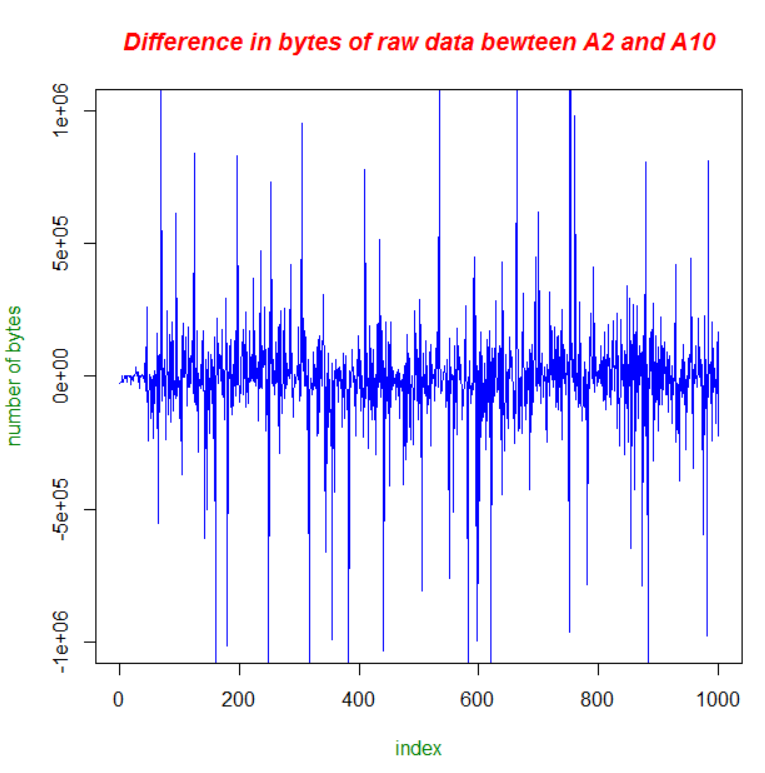
\includegraphics[scale=0.55, keepaspectratio=true]{figures/q4.PNG}
\caption{Output graph with difference in bytes of raw data}
\label{fig:q4fig1}
\end{center}
\end{figure}
\item The output graph where the y-axis corresponds to the difference in bytes of the processed data is illustrated in Figure \ref{fig:q4fig2}. 
\begin{figure}[h!]
\begin{center}
\hspace*{-3cm} 
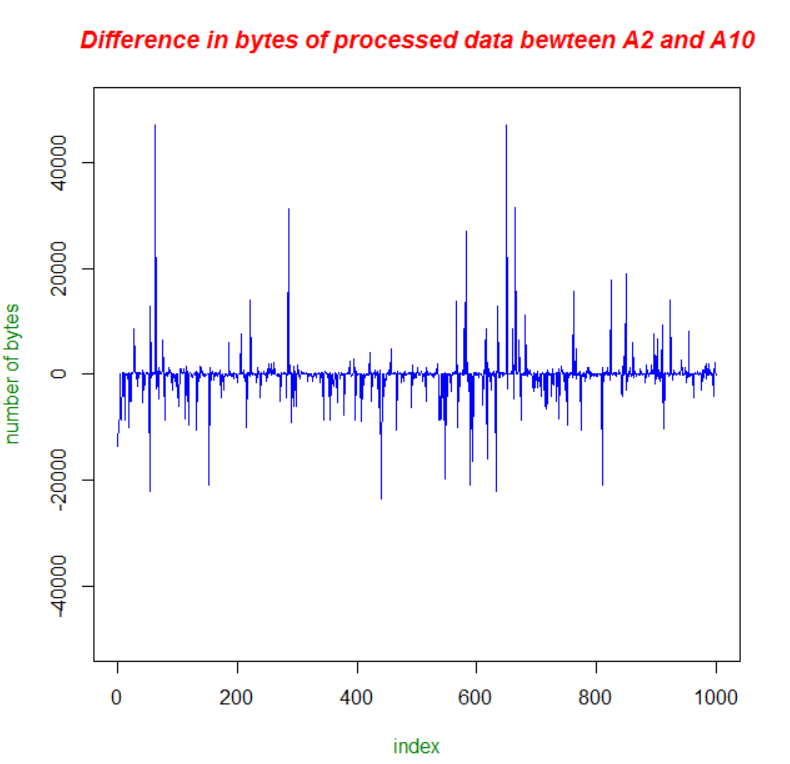
\includegraphics[scale=0.55, keepaspectratio=true]{figures/q4p.PNG}
\caption{Output graph with difference in bytes of processed data}
\label{fig:q4fig2}
\end{center}
\end{figure}
\end{itemize}

\newpage
\textbf{Code Listing}
\sloppy
\lstinputlisting[language=Python,caption= Python code for finding count for each status code,frame=single,breaklines=true,label=lst:q4code1, tabsize=2, captionpos=b,numbers=left,showspaces=false,showstringspaces=false,basicstyle=\footnotesize]{src/checkRedirect.py}


\textbf{Code Listing}
\sloppy
\lstinputlisting[language=Python,caption=python code for getting processed data for each blog URI,frame=single,breaklines=true,label=lst:q4code2, tabsize=2, captionpos=b,numbers=left,showspaces=false,showstringspaces=false,basicstyle=\footnotesize]{src/RawData.py}


\textbf{Code Listing}
\sloppy
\lstinputlisting[language=Python,caption=python code for getting raw data for each blog URI,frame=single,breaklines=true,label=lst:q4code3, tabsize=2, captionpos=b,numbers=left,showspaces=false,showstringspaces=false,basicstyle=\footnotesize]{src/ProcessedData.py}


\textbf{Code Listing}
\sloppy
\lstinputlisting[language=Python,caption= Python code for getting bytes of each blog file in raw data and processed data,frame=single,breaklines=true,label=lst:q4code4, tabsize=2, captionpos=b,numbers=left,showspaces=false,showstringspaces=false,basicstyle=\footnotesize]{src/getBytes.py}


\textbf{Code Listing}
\sloppy
\lstinputlisting[language=Python,caption=python code for getting difference between bytes of raw/processed data in assignmnet 2 and assignment 10,frame=single,breaklines=true,label=lst:q4code5, tabsize=2, captionpos=b,numbers=left,showspaces=false,showstringspaces=false,basicstyle=\footnotesize]{src/getDifference1.py}

